\documentclass{article}
\usepackage{icml2026}

% ------------------------------------------------------------
% Packages
% ------------------------------------------------------------
\usepackage[utf8]{inputenc}
\usepackage{amsmath,amssymb,amsthm,amsfonts}
\usepackage{algorithm}
\usepackage{algorithmic}
\usepackage{graphicx}
\usepackage{subcaption}
\usepackage{booktabs}
\usepackage{float}
\usepackage{natbib}
\usepackage{enumitem}
\usepackage{mathtools}
\usepackage{tikz}
\usepackage{pgfplots}
\usepackage{fontspec}
\usepackage[english,provide=*]{babel}
\usepackage{changepage}
\usepackage{pgfplots}
\usepgfplotslibrary{groupplots}


\pgfplotsset{compat=1.18}

% ------------------------------------------------------------
% Theorem environments
% ------------------------------------------------------------
\newtheorem{theorem}{Theorem}
\newtheorem{proposition}{Proposition}
\newtheorem{lemma}{Lemma}
\newtheorem{remark}{Remark}

% ------------------------------------------------------------
% Macros
% ------------------------------------------------------------
\babelprovide[import,onchar=ids fonts]{english}
\babelprovide[onchar=ids fonts]{tifinagh}
% Standard Latin Modern is the default for fontspec if no other font is set.
% We only define the font for Tifinagh.
\babelfont[tifinagh]{rm}{Ebrima}

% Robust \yat definition with fallback
\newfontfamily\tifinaghfont{Noto Sans Tifinagh}
\DeclareRobustCommand{\E}{\text{\normalfont\tifinaghfont ⵟ}}

\newcommand{\R}{\mathbb{R}}
\newcommand{\Sph}{\mathbb{S}}
\newcommand{\norm}[1]{\left\lVert #1 \right\rVert}
\newcommand{\inner}[2]{\left\langle #1, #2 \right\rangle}

% ------------------------------------------------------------
% Title / Authors
% ------------------------------------------------------------

\begin{document}

\twocolumn[
\icmltitle{SLAY:\\
Spherical Linearized Attention with Yat-Kernel}
\icmltitlerunning{SLAY: Spherical Linearized Attention with Yat-Kernel}

\begin{icmlauthorlist}
\icmlauthor{Jose Miguel Luna}{equal}
\icmlauthor{Taha Bouhsine}{equal}
\icmlauthor{Krzysztof Choromanski}{}
\end{icmlauthorlist}

\icmlaffiliation{equal}{Anonymous Institution}
\icmlcorrespondingauthor{Anonymous}{anon.email@domain.com}

\icmlkeywords{Linear Attention, Neural Matter Networks, Random Features, Long Context}

\vskip 0.3in
]

\printAffiliationsAndNotice{}

% ------------------------------------------------------------
% Abstract
% ------------------------------------------------------------
\begin{abstract}
The Yat-product operator $\E(q,k)$ yields geometry-aware interactions but leads to quadratic $O(L^2)$ attention due to a non-factorizable denominator. We introduce \emph{SLAY} (\emph{Spherical Linearized Attention with YAT-Kernels}), which constrains queries and keys to the unit sphere so the kernel depends only on angular alignment. Using Bernstein’s theorem, we express the spherical YAT kernel as a nonnegative mixture of polynomial--exponential product kernels and derive a strictly positive random-feature approximation with linear-time $O(L)$ attention. We prove positive definiteness and boundedness on the sphere and show the estimator yields nonnegative scores with a positive denominator under mild conditions. Empirically, SLAY matches full spherical YAT attention and compares favorably to linearized baselines on language modeling and image classification while retaining linear scaling in $L$.
\end{abstract}

% ============================================================
% 1. Introduction
% ============================================================
\section{Introduction}
\label{sec:intro}

Transformer models owe much of their success to attention, which enables dynamic, content-dependent interactions between tokens. In standard Transformers, attention is implemented via softmax applied to pairwise query--key similarities. While expressive, this requires constructing an explicit $L \times L$ attention matrix for a sequence of length $L$, resulting in quadratic time and memory complexity. This cost rapidly becomes prohibitive as context lengths grow, fundamentally limiting long-context modeling.

To overcome this bottleneck, \emph{linear attention} mechanisms reinterpret attention as kernel evaluation and exploit feature maps to reorder computation. Early examples include kernelized Transformers \citep{katharopoulos2020transformers} and random-feature approximations of the softmax kernel \citep{choromanski2021}. These works show that positive random features can yield stable and scalable attention for specific kernels.

Our approach linearizes the spherical \E-product kernel directly rather than applying a softmax to it, and uses positivity-preserving approximations to ensure stable kernel normalization.

Despite these advances, softmax attention remains tied to a specific similarity: the exponential of an inner product. This choice conflates alignment and magnitude, and its unbounded growth requires careful normalization and stabilization. These limitations motivate alternative attention kernels that are geometrically grounded, self-regularizing, and compatible with efficient computation, as explored in activation-free architectures \citep{nmn2026}.

Neural Matter Networks (NMNs) introduced the \emph{\E-Product} (also referred to as the Yat-product) \citep{nmn2026}, a kernel operator inspired by inverse-square interactions in physics:
\begin{equation}
\E(q,k) = \frac{(q^\top k)^2}{\|q-k\|^2 + \epsilon}
\label{eq:eproduct}
\end{equation}
where $\epsilon > 0$ ensures numerical stability. Unlike standard dot-product similarity, the \E-Product explicitly couples two geometric quantities: \emph{alignment} and \emph{proximity}. The squared inner product in the numerator yields an even (sign-symmetric) alignment score, while the inverse-distance denominator penalizes interactions between distant vectors. This ratio yields a self-regularizing response that can suppress irrelevant interactions without requiring explicit activation functions or normalization layers.

From a theoretical perspective, the \E-Product can be viewed as a kernel-like similarity operator. NMNs constructed as linear combinations of \E-Product units are universal approximators on compact domains, despite being entirely activation-free \citep{nmn2026}. In this work, we focus on a unit-norm (spherical) setting where the resulting isotropic kernel admits a clean positive-definiteness proof and stable, bounded responses.

In the context of attention, the \E-Product offers a geometry-aware alternative to softmax similarity. It favors tokens that are both aligned and close in representation space. However, the same geometric coupling introduces a computational obstacle: the denominator $\|q-k\|^2 = \|q\|^2 + \|k\|^2 - 2q^\top k$ entangles query and key terms and prevents the factorization required for efficient linear attention. As a result, naive \E-Product attention still requires explicit pairwise interactions and reverts to quadratic complexity. This mirrors the general limitation for non-factorizable kernels that motivates linearization techniques such as those used in Performer \citep{choromanski2021}.

This paper addresses this limitation for \E-Attention. We show that by constraining queries and keys to lie on the unit sphere and reformulating the resulting kernel using Bernstein’s theorem, the \E-Product admits a nonnegative mixture representation that can be approximated by strictly positive random features. This yields a linear-time attention mechanism that preserves the core geometric and self-regulating properties of the \E-Product while enabling scalable long-context Transformers.

\paragraph{Contributions.}
We introduce SLAY (\textbf{Spherical YAT-Attention}), a geometry-aware attention mechanism, with the following characteristics:
\begin{itemize}[leftmargin=1.4em]
\item Enforces unit-norm constraints on queries and keys, decoupling alignment and distance.
\item Linearizes the spherical \E-product via an integral representation based on Bernstein’s theorem.
\item Approximates the resulting kernel using strictly positive Tensor Product Random Features.
\item Achieves linear-time $O(L)$ attention while preserving key theoretical properties of NMNs.
\end{itemize}

% ============================================================
% 2. Methodology
% ============================================================
\section{Methodology}
\label{sec:method}

Our goal is to compute \E-attention with the spherical \E-product kernel from Eq.~\eqref{eq:spherical} without forming the $L\times L$ matrix of pairwise interactions.
We first normalize queries/keys to the unit sphere so the kernel depends only on $x=\hat q^\top \hat k\in[-1,1]$. We then linearize the non-factorizable term $1/(C-2x)$ via a Laplace integral (Bernstein's theorem), discretize the resulting nonnegative mixture using Gauss--Laguerre quadrature, and approximate each product kernel with strictly positive random features. Finally, we apply the standard kernel-attention reordering using the resulting feature map $\widetilde{\Psi}(\cdot)$.

Throughout this work, we approximate the spherical \E-product (YAT) kernel itself; normalization is performed via kernel sums as in linear attention, not via a softmax nonlinearity.

\subsection{Spherical Constraint}

We assume $d \ge 2$ throughout, where spherical isotropy theory applies. We normalize inputs to the unit sphere:
\[
\hat q = \frac{q}{\|q\|}, \qquad \hat k = \frac{k}{\|k\|}, \qquad \|\hat q\|=\|\hat k\|=1.
\]
Expanding the denominator of Eq.~\eqref{eq:eproduct} yields:
\begin{align}
\|\hat q-\hat k\|^2 + \epsilon
&= \|\hat q\|^2 + \|\hat k\|^2 - 2\hat q^\top \hat k + \epsilon \\
&= (2+\epsilon) - 2\hat q^\top \hat k.
\end{align}
Let $x=\hat q^\top \hat k\in[-1,1]$ and $C=2+\epsilon$. The spherical \E-product becomes
\begin{equation}
\E_{\text{sph}}(\hat q,\hat k)
= \frac{x^2}{C-2x}.
\label{eq:spherical}
\end{equation}
Thus, the kernel depends only on angular alignment.

\paragraph{Geometric intuition.}
On the unit sphere $\Sph^{d-1}$, the squared \emph{chordal} distance is
\[
d_{\Sph^{d-1}}(\hat q, \hat k)^2 = 2(1 - \hat q^\top \hat k),
\]
so the spherical \E-product can be written as a distance-regularized alignment score:
\begin{equation}
\E_{\mathrm{sph}}(\hat q, \hat k) = \frac{\langle \hat q, \hat k \rangle^2}{d_{\Sph^{d-1}}(\hat q, \hat k)^2 + \epsilon}.
\label{eq:geometric}
\end{equation}
Additional discussion (including invariances and the connection to isotropic spherical kernels \citep{schoenberg1942}) is deferred to Appendix~\ref{app:geom}.

\subsection{Integral Linearization}
The function $g(y) = 1/y$ is completely monotone on $(0,\infty)$, which by Bernstein's theorem implies the Laplace representation $1/y = \int_0^\infty e^{-sy}\,ds$ \citep{widder1941laplace,schilling2012}. To apply this identity to our kernel, we substitute $y = C - 2x$ and verify that $y > 0$ for all $x \in [-1,1]$.

Since $x \le 1$ and $C=2+\epsilon$, we have $y=C-2x \ge \epsilon > 0$, hence Bernstein's representation applies on the full domain (see Lemma~\ref{lem:complete-monotone} in Appendix~\ref{app:background}).


Using Bernstein’s theorem for completely monotone functions, a standard tool in kernel analysis previously used to construct positive random feature approximations for exponential kernels \citep{choromanski2021},
\begin{equation}
\frac{1}{y} = \int_0^\infty e^{-sy}\,ds,
\end{equation}
we obtain
\begin{align}
\E_{\text{sph}}(\hat q,\hat k)
&= x^2 \int_0^\infty e^{-s(C-2x)}ds \\
&= \int_0^\infty e^{-sC}\,\Big[x^2 e^{2s x}\Big]\,ds.
\label{eq:integral}
\end{align}
This expresses the spherical \E-product as a positively weighted mixture of product kernels:
namely, a degree-2 polynomial factor $(\hat q^\top \hat k)^2$ multiplied by an exponential dot-product kernel $e^{2s\,\hat q^\top \hat k}$.

Importantly, the factor $x^2$ cannot be absorbed into a \emph{nonnegative} Laplace weight over plain exponentials without introducing signed correction terms (see Appendix~\ref{app:features}).

This representation is analogous to the Laplace-transform-based decompositions used to derive unbiased positive random feature estimators for softmax and Gaussian kernels \citep{choromanski2021}.

\subsection{Kernel Approximation and Positive Features}

\subsubsection{Quadrature (Gauss--Laguerre)}

We approximate the integral in Eq.~\eqref{eq:integral} using $R$-point Gauss--Laguerre quadrature. We apply Gauss--Laguerre quadrature after the change of variables $t = Cs$, so that $\int_0^\infty e^{-Cs} h(s)\,ds = \frac{1}{C}\int_0^\infty e^{-t} h(t/C)\,dt$:
\[
\int_0^\infty e^{-sC} h(s)\,ds \;\approx\; \sum_{r=1}^R w_r\, h(s_r),
\]
where $\{t_r,\alpha_r\}_{r=1}^R$ are the standard Gauss--Laguerre nodes and weights for $\int_0^\infty e^{-t}f(t)\,dt$ and
\[
s_r=\frac{t_r}{C},\qquad w_r=\frac{\alpha_r}{C}.
\]
Thus, the $w_r$ already incorporate the $1/C$ factor induced by $t=Cs$. Since $|x| \le 1$, the integrand $h(s) = x^2 e^{2sx}$ is entire and uniformly bounded by $e^{2s}$, ensuring uniform exponential convergence over $x \in [-1,1]$. Such bounds follow from classical results on Gauss--Laguerre quadrature for entire functions of exponential type (see Theorem 3.6.24 in \citep{davis1984,gautschi2004}); for a shapes/implementation summary, see Appendix~\ref{app:impl}.

\subsubsection{Random features (polynomial and exponential)}

\paragraph{Polynomial component and approximations.}
For the exact polynomial kernel $(\hat q^\top \hat k)^2$, the explicit feature map $\phi_{\text{poly}}(u) = \mathrm{vec}(u u^\top) \in \R^{d^2}$ yields exact reconstruction:
\[
\langle \phi_{\text{poly}}(\hat q), \phi_{\text{poly}}(\hat k) \rangle = (\hat q^\top \hat k)^2.
\]
In practice, we reduce dimensionality via low-dimensional approximations. We consider TensorSketch \citep{pham2013} as well as three common approximations to the degree-2 polynomial kernel $k_{\text{poly}}(x,y)=(x^\top y)^2$, described formally in Appendix~\ref{app:prelim-poly}: (i) Random Maclaurin (RM) features \citep{karkarnick2012}, (ii) Nystr"om features using anchor points \citep{williams2001nystrom}, and (iii) anchor features using squared inner products to fixed anchors.

\paragraph{Anchor features.}
Let anchors $\{a_i\}_{i=1}^P\subset\R^d$ be fixed reference vectors. Anchor features define
\[
\phi_{\mathrm{anc}}(x) = \frac{1}{\sqrt{P}}\bigl[(x^\top a_i)^2\bigr]_{i=1}^P,
\]
yielding a simple low-rank approximation whose induced inner products are nonnegative.

Unlike Nystr"om approximations, anchor features do not require inversion/whitening of the anchor Gram matrix and therefore preserve non-negativity of approximate kernel evaluations.

\paragraph{Default choice.}
Unless stated otherwise, we use \emph{anchor features} as the default polynomial approximation because they (i) preserve non-negativity of the polynomial component (supporting the denominator-positivity guarantees), (ii) are empirically stable at small feature budgets, and (iii) are computationally simple ($O(dP)$ per token). The multi-scale sweep in Table~\ref{tab:poly-sweep} (Appendix~\ref{app:poly-ablation}) supports this choice.

Table~\ref{tab:poly-approximations} summarizes the trade-offs between polynomial approximations, highlighting positivity preservation as a key distinction.

\begin{table*}[t]
\centering
\small
\caption{Polynomial kernel approximation options for $(x^\top y)^2$. Here $D_p$ denotes the polynomial-feature dimension, and $P$ denotes the number of anchors (when applicable). \emph{Feature cost} is the asymptotic cost of computing the polynomial features for one vector and excludes quadrature/PRF computation, tensor-product fusion/sketching, and the linear-attention contractions; these additional costs drive end-to-end latency in Section~\ref{sec:experiments}.}
\label{tab:poly-approximations}
\begin{tabular*}{\textwidth}{@{\extracolsep{\fill}}lcccc}
\toprule
Method & Dim. & Feature cost & Unbiased? & $\langle\phi(x),\phi(y)\rangle\ge 0$? \\
\midrule
Exact $\mathrm{vec}(uu^\top)$ & $d^2$ & $O(d^2)$ & Yes & Yes \\
TensorSketch \citep{pham2013} & $D_p$ & $\approx O(d + D_p\log D_p)$ & Approx. & No (not guaranteed) \\
Random Maclaurin \citep{karkarnick2012} & $D_p$ & $O(d\,D_p)$ & Yes & No (not guaranteed) \\
Nystr\"om \citep{williams2001nystrom} & $P$ & $O(d\,P)$ & Approx. & No (not guaranteed) \\
Anchor features (low-rank) \citep{scholkopf2002learning} & $P$ & $O(d\,P)$ & No & Yes \\
\bottomrule
\end{tabular*}
\end{table*}

For the theoretical non-negativity and denominator-positivity guarantees stated later, we require a polynomial component whose induced score estimates are nonnegative (e.g., the exact map, or anchor features). Signed polynomial approximations (TensorSketch, Random Maclaurin) and Nystr"om features can yield negative approximate inner products and are therefore treated as accuracy/efficiency baselines rather than positivity-guaranteeing estimators.

\paragraph{Why the polynomial factor is needed for fidelity.}
The $x^2$ factor in Eq.~\eqref{eq:integral} is part of the target kernel; removing it yields a different kernel (see Appendix~\ref{app:features}).

Retaining the polynomial factor is essential both for kernel fidelity and for positivity guarantees of the resulting attention scores.

\paragraph{Positive Random Features.}
For the exponential term $e^{2s\,\hat q^\top \hat k}$, we use Positive Random Features applied to the \emph{original normalized vectors}:
\begin{equation}
\phi_{\text{PRF}}(u; s)
=
\frac{1}{\sqrt{D}}
\left[
\exp\!\left(\sqrt{2s}\,\omega_i^\top u - s\right)
\right]_{i=1}^D,
\end{equation}
where $\omega_i \sim \mathcal{N}(0, I_d)$ are drawn independently.
This construction satisfies
\[
\mathbb{E}\!\left[
\langle \phi_{\text{PRF}}(\hat q; s),
\phi_{\text{PRF}}(\hat k; s) \rangle
\right]
=
e^{2s\,\hat q^\top \hat k}
\]
for unit-norm inputs (a standard positive random feature identity for exponential dot-product kernels; see \citep{choromanski2021} and Proposition~\ref{prop:prf-unbiased} in Appendix~\ref{app:background}).

\subsubsection{Fusing polynomial and PRF features}

\paragraph{Fusion.}
Since the polynomial and PRF feature maps are applied to vectors (not scalars), we obtain for each scale $r$:
\begin{equation}
\widetilde{\Psi}_r(u)
=
\sqrt{w_r}\,\mathcal{S}\Bigl(\phi_{\text{poly}}(u)\otimes \phi_{\text{PRF}}(u; s_r)\Bigr),
\end{equation}
where $\mathcal{S}:\R^{D_pD_r}\to\R^{D_t}$ is a (randomized) sketching operator that approximates the tensor-product feature map without explicitly materializing the $D_pD_r$-dimensional Kronecker vector.
We then define $\widetilde{\Psi}(u)$ as the concatenation over $r=1,\dots,R$.

Conceptually, the target kernel at each quadrature node is the product kernel $(\hat q^\top \hat k)^2\,e^{2s_r\hat q^\top \hat k}$, whose RKHS is the tensor product $\mathcal{H}_{\text{poly}}\otimes\mathcal{H}_{\exp,s_r}$. The sketching operator $\mathcal{S}$ provides a computationally efficient approximation of this tensor-product feature map.

\begin{adjustwidth}{1.5em}{1.5em}
\begin{remark}[Feature Map Target]
\label{rem:feature-target}
$\widetilde{\Psi}$ targets the \emph{integrand} $k_s(x)=x^2 e^{2sx}$; consequently,
\[
\mathbb{E}[\langle \widetilde{\Psi}(\hat q), \widetilde{\Psi}(\hat k) \rangle] \approx \sum_{r=1}^R w_r\,(\hat q^\top \hat k)^2 e^{2s_r\hat q^\top \hat k},
\]
which is a quadrature approximation to Eq.~\eqref{eq:integral}.
\end{remark}
\end{adjustwidth}

\begin{adjustwidth}{1.5em}{1.5em}
\begin{remark}[Bias Decomposition]
\label{rem:bias}
$\langle \widetilde{\Psi}(\hat q), \widetilde{\Psi}(\hat k) \rangle$ is unbiased for the discretized (quadrature) kernel, but biased for the true kernel unless $R\to\infty$.
\end{remark}
\end{adjustwidth}

\subsection{Linear-Time Attention Computation}

Given $Q,K,V\in\R^{L\times d}$, we compute normalized inputs, apply $\Psi$, and use the standard linear-attention reordering:
\[
\hat Y = \frac{\widetilde{\Psi}(Q)\big(\widetilde{\Psi}(K)^\top V\big)}
{\widetilde{\Psi}(Q)\big(\widetilde{\Psi}(K)^\top \mathbf{1}\big)}.
\]
Note that this normalization is not a softmax; it corresponds to kernel normalization and preserves linear-time computation.
Here the division is applied row-wise (broadcast across the value dimension); in practice we add a small stabilizer $\delta>0$ to the denominator for numerical stability \citep{higham2002}. Concretely, if $\Psi(Q),\Psi(K)\in\R^{L\times m}$ (feature dimension $m$) and $V\in\R^{L\times d_v}$, then $\Psi(K)^\top V\in\R^{m\times d_v}$, $\Psi(K)^\top\mathbf{1}\in\R^{m\times 1}$, and the denominator is an $L\times 1$ vector broadcast over $d_v$ (see Appendix~\ref{app:impl}).

\begin{algorithm}[t]
\caption{Spherical \E-Attention Forward Pass}
\begin{algorithmic}[1]
\REQUIRE $Q,K,V\in\R^{L\times d}$
\STATE Normalize $Q,K$ to unit norm
\STATE Compute polynomial features $\phi_{\text{poly}}(Q),\phi_{\text{poly}}(K)$ (e.g., anchor features by default)
\FOR{$r=1$ to $R$}
\STATE Compute PRF features $\phi_{\text{PRF}}(\cdot; s_r)$
\STATE Fuse features via sketched tensor product $\widetilde{\Psi}_r$
\ENDFOR
\STATE Concatenate features $\widetilde{\Psi}(Q),\widetilde{\Psi}(K)$
\STATE Compute numerator and denominator
\RETURN $\hat Y$
\end{algorithmic}
\end{algorithm}

\paragraph{Complexity.}
Let $m$ denote the final feature dimension (after concatenating across $R$ quadrature nodes), which in our construction scales as $m=O(RD_t)$. The linear-attention contractions cost $O(L\,m\,d_v)$ time and $O(L\,m)$ space (the $L\times L$ attention matrix is never formed).
Feature construction depends on the polynomial approximation: exact degree-2 features cost $O(L\,d^2)$, anchor features cost $O(L\,dP)$, Random Maclaurin costs $O(L\,dD_p)$, and TensorSketch costs approximately $O(L\,(d + D_p\log D_p))$ per layer.
The PRF exponential features contribute $O(L\,R\,dD)$ time. Appendix~\ref{app:impl} collects practical knob choices and shape details.
See Appendix~\ref{app:impl} for explicit tensor-product scaling (without sketching) and causal-vs.-non-causal implementation notes.


% ------------------------------------------------------------
% 7. Experiments
% ------------------------------------------------------------
\section{Experiments}
\label{sec:experiments}

We evaluate SLAY along several axes. First, we analyze polynomial approximation options to identify optimal configurations. Second, we benchmark computational costs by measuring latency, memory, and throughput scaling with sequence length. Third, we evaluate SLAY on 22 synthetic tasks spanning core capabilities and higher-level behaviors. Fourth, we assess the linear approximation quality of SLAY against standard attention. Fifth, we conduct an extreme classification test to evaluate performance under challenging conditions. Finally, we train 2.5B parameter transformers to compare SLAY against both quadratic and linear complexity attention mechanisms.

Unless stated otherwise, all variants share the same architecture and training settings; we change only the attention operator and its feature configuration.

\subsection{Ablation: Polynomial and Attention Approximation}
\label{subsec:poly-ablation}


\paragraph{Polynomial Approximation}
We isolate the polynomial factor $(\hat q^\top \hat k)^2$ and compare several approximations (anchor, Nystr\"om, TensorSketch, Random Maclaurin). We report (i) kernel-normalized attention output error relative to exact spherical \E-attention and (ii) forward-pass latency, under matched feature budgets; protocol details and the multi-scale sweep are in Appendix~\ref{app:experiments} and Table~\ref{tab:poly-sweep} (Appendix~\ref{app:poly-ablation}).

For reference, we also include Laplace-only and a Hadamard-fusion variant. These are not polynomial approximations of $(\hat q^\top \hat k)^2$: they change the estimator by removing or altering the polynomial factor. Under feature-budget matching, they can therefore require substantially larger PRF feature dimension to reach comparable overall feature counts, which can dominate runtime.

At the large scale (Table~\ref{tab:poly-ablation-snapshot}), anchor and Laplace-only achieve the lowest errors, but anchor is markedly faster (\,$489$ ms vs.~$1906$ ms\,) and is our default choice in the remaining experiments. Nystr\"om is substantially less accurate at these budgets. Signed polynomial approximations (TensorSketch and Random Maclaurin) can yield negative approximate inner products, leading to denominator cancellation and severe instability; we include them as efficiency baselines rather than positivity-guaranteeing estimators.

\begin{table}[t]
\centering
\small
\caption{Polynomial-approximation ablation (large-scale snapshot; see the ``Large'' block in Table~\ref{tab:poly-sweep}). Lower Rel.~$\ell_2$ is better; latency is forward-pass time under the same feature-budget matching across methods (which can increase PRF dimensionality for Laplace-only/Hadamard). Very large errors indicate severe kernel mismatch/instability. Full multi-scale sweep is in Table~\ref{tab:poly-sweep} (Appendix~\ref{app:poly-ablation}).}
% Note: these latencies include the full attention pipeline (PRF/quadrature, fusion/sketching, and contractions), not just polynomial feature construction.
\label{tab:poly-ablation-snapshot}
\begin{tabular}{lcc}
\toprule
Method & Rel.~$\ell_2\downarrow$ & Latency (ms)$\downarrow$ \\
\midrule
Exact (Spherical) & 0.0000 & 5.02 \\
Laplace-only & 0.4850 & 1905.80 \\
Anchor & 0.4939 & 489.42 \\
Hadamard (shared $\omega$) & 0.6793 & 1932.07 \\
Nystr\"om & 28.1970 & 569.64 \\
TensorSketch & $4.62\times 10^5$ & 547.76 \\
Random Maclaurin & $1.77\times 10^6$ & 551.43 \\
\bottomrule
\end{tabular}
\end{table}

\paragraph{Attention Approximation Errors}

\subsection{Computational Costs}
\label{subsec:computational-costs}

We compare the computational efficiency of \textbf{SLAY}, a linearized estimator of spherical YAT attention, against both quadratic and linear attention mechanisms. We report latency, peak memory usage, and throughput as functions of sequence length, focusing on regimes relevant to long-context modeling.

\paragraph{Benchmark setup.}
All attention mechanisms are benchmarked in isolation using a causal attention kernel with identical architectural settings (embedding dimension 256, 8 heads, batch size 1). Experiments are conducted on a single NVIDIA A100-SXM4 GPU (80\,GB). For each sequence length, we report mean latency over multiple timed runs after warm-up, peak GPU memory allocation, and effective throughput measured in tokens per second. Sequence lengths range from 128 tokens up to 131K tokens, or until out-of-memory (OOM) failure.

\paragraph{Results overview.}
Figures~\ref{fig:latency-scaling}--\ref{fig:throughput-scaling} summarize the scaling behavior. Quadratic attention mechanisms (standard softmax and exact YAT) exhibit rapidly increasing latency and memory usage, failing beyond 16K tokens. In contrast, linear attention methods scale approximately linearly and remain stable up to 128K tokens.


\begin{figure}[htbp]
\centering
\caption{Attention mechanisms scaling behaviors.}
\label{fig:scaling}
\vspace{0.3em}

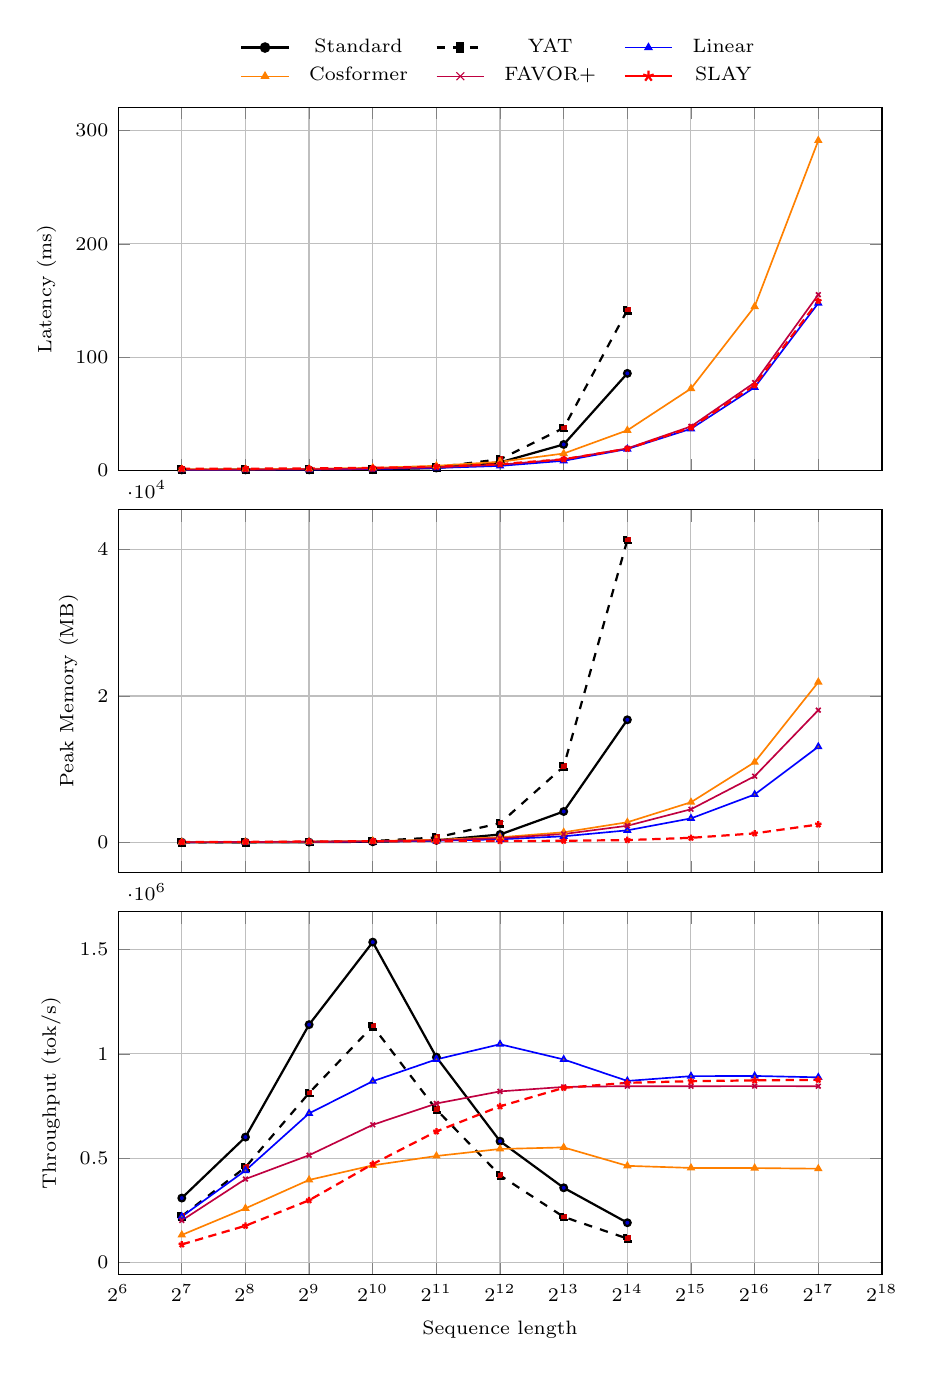
\begin{tikzpicture}

% ================== Legend ==================
\begin{axis}[
    hide axis,
    xmin=0, xmax=1,
    ymin=0, ymax=1,
    width=\columnwidth*.8,
    height=0.38\columnwidth,
    scale only axis,
    legend columns=3,
    legend style={
        font=\scriptsize,
        at={(0.5,1.03)}, 
        anchor=south,
        draw=none,
        column sep=0.5em,
        /tikz/every even column/.append style={column sep=0.8em}
    },
]
\addlegendimage{black, thick, mark=*, mark size=1.5pt}
\addlegendentry{Standard}
\addlegendimage{black, dashed, thick, mark=square*, mark size=1.5pt}
\addlegendentry{YAT}
\addlegendimage{blue, mark=triangle*, mark size=1.5pt}
\addlegendentry{Linear}
\addlegendimage{orange, mark=triangle*, mark size=1.5pt}
\addlegendentry{Cosformer}
\addlegendimage{purple, mark=x, mark size=2pt}
\addlegendentry{FAVOR+}
\addlegendimage{red, thick, mark=star, mark size=2pt}
\addlegendentry{SLAY}
\end{axis}

% ================== Grouped plots ==================
\begin{groupplot}[
    group style={
        group size=1 by 3,
        vertical sep=0.5cm,
    },
    width=\columnwidth*.8,
    height=0.38\columnwidth,
    xmode=log,
    log basis x=2,
    scale only axis,
    grid=both,
    grid style={line width=0.3pt, gray!30},
    major grid style={line width=0.4pt, gray!50},
    tick label style={font=\scriptsize},
    label style={font=\scriptsize},
    every axis plot/.append style={line width=0.6pt, mark size=1.2pt},
]

% ================== (a) Latency ==================
\nextgroupplot[
    ylabel={Latency (ms)},
    xticklabels={},
    ymin=0,
]

\addplot+[black, thick, mark=*] coordinates {
(128,0.41) (256,0.43) (512,0.45) (1024,0.67)
(2048,2.08) (4096,7.04) (8192,22.84) (16384,85.60)
};
\addplot+[black, dashed, thick, mark=square*] coordinates {
(128,0.57) (256,0.56) (512,0.63) (1024,0.90)
(2048,2.79) (4096,9.79) (8192,37.38) (16384,141.43)
};
\addplot+[blue, mark=triangle*] coordinates {
(128,0.58) (256,0.58) (512,0.72) (1024,1.18)
(2048,2.10) (4096,3.91) (8192,8.42) (16384,18.82)
(32768,36.68) (65536,73.27) (131072,147.63)
};
\addplot+[orange, mark=triangle*] coordinates {
(128,0.96) (256,0.98) (512,1.29) (1024,2.20)
(2048,4.01) (4096,7.52) (8192,14.84) (16384,35.32)
(32768,72.19) (65536,144.60) (131072,291.17)
};
\addplot+[purple, mark=x] coordinates {
(128,0.63) (256,0.64) (512,0.99) (1024,1.55)
(2048,2.69) (4096,4.99) (8192,9.73) (16384,19.38)
(32768,38.77) (65536,77.48) (131072,155.06)
};
\addplot+[red, thick, mark=star] coordinates {
(128,1.46) (256,1.45) (512,1.71) (1024,2.17)
(2048,3.26) (4096,5.47) (8192,9.78) (16384,19.02)
(32768,37.69) (65536,75.05) (131072,149.63)
};

% ================== (b) Memory ==================
\nextgroupplot[
    ylabel={Peak Memory (MB)},
    xticklabels={},
]

\addplot+[black, thick, mark=*] coordinates {
(128,11.9) (256,15.7) (512,29.4) (1024,81.1)
(2048,282.1) (4096,1074.1) (8192,4218.1) (16384,16746.1)
};
\addplot+[black, dashed, thick, mark=square*] coordinates {
(128,13.4) (256,21.7) (512,53.4) (1024,177.2)
(2048,666.3) (4096,2610.4) (8192,10362.6) (16384,41323.1)
};
\addplot+[blue, mark=triangle*] coordinates {
(128,22.9) (256,35.6) (512,61.1) (1024,112.1)
(2048,214.1) (4096,418.1) (8192,826.1) (16384,1642.1)
(32768,3274.1) (65536,6538.1) (131072,13066.1)
};
\addplot+[orange, mark=triangle*] coordinates {
(128,31.5) (256,52.9) (512,95.6) (1024,181.1)
(2048,352.2) (4096,694.2) (8192,1378.2) (16384,2746.3)
(32768,5482.5) (65536,10954.9) (131072,21899.6)
};
\addplot+[purple, mark=x] coordinates {
(128,27.8) (256,45.4) (512,80.7) (1024,151.2)
(2048,292.3) (4096,574.3) (8192,1138.4) (16384,2266.7)
(32768,4523.2) (65536,9036.2) (131072,18062.2)
};
\addplot+[red, thick, mark=star] coordinates {
(128,36.2) (256,62.2) (512,114.2) (1024,151.7)
(2048,160.7) (4096,178.7) (8192,214.7) (16384,314.2)
(32768,618.2) (65536,1226.2) (131072,2442.2)
};

% ================== (c) Throughput ==================
\nextgroupplot[
    ylabel={Throughput (tok/s)},
    xlabel={Sequence length},
]

\addplot+[black, thick, mark=*] coordinates {
(128,309605) (256,601515) (512,1140190) (1024,1535463)
(2048,984540) (4096,581929) (8192,358680) (16384,191393)
};
\addplot+[black, dashed, thick, mark=square*] coordinates {
(128,223026) (256,457217) (512,812948) (1024,1132992)
(2048,733302) (4096,418302) (8192,219174) (16384,115845)
};
\addplot+[blue, mark=triangle*] coordinates {
(128,220935) (256,441509) (512,715210) (1024,869111)
(2048,973777) (4096,1046247) (8192,973413) (16384,870581)
(32768,893397) (65536,894465) (131072,887852)
};
\addplot+[orange, mark=triangle*] coordinates {
(128,132910) (256,260132) (512,396415) (1024,466298)
(2048,511045) (4096,544607) (8192,552194) (16384,463905)
(32768,453914) (65536,453236) (131072,450163)
};
\addplot+[purple, mark=x] coordinates {
(128,202368) (256,400720) (512,514787) (1024,660425)
(2048,762536) (4096,820486) (8192,841800) (16384,845487)
(32768,845161) (65536,845833) (131072,845286)
};
\addplot+[red, thick, mark=star] coordinates {
(128,87397) (256,176813) (512,299006) (1024,472417)
(2048,628732) (4096,748980) (8192,837345) (16384,861529)
(32768,869331) (65536,873279) (131072,875953)
};

\end{groupplot}
\end{tikzpicture}
\end{figure}

SLAY closely follows the scaling behavior of other linear attention mechanisms while substantially reducing memory usage relative to exact spherical YAT attention. At long sequence lengths, SLAY sustains high throughput comparable to other linear baselines, demonstrating that its added geometric structure does not compromise scalability.

\begin{table}[htbp]
\centering
\small
\caption{Kernel approximation quality. Rel.~$\ell_2$ is relative L2 error (lower is better), Cos is cosine similarity (higher is better).}
\label{tab:kernel-quality}
\begin{tabular}{lccc}
\toprule
Method & Rel.~$\ell_2\downarrow$ & Cos$\uparrow$ & MSE$\downarrow$\\
\midrule
yat-performer-anchor & 0.5275 & 0.8496 & 4.55e-03\\
yat-performer-laplace & 0.5440 & 0.8391 & 4.84e-03\\
yat-performer & 0.7894 & 0.7321 & 1.02e-02\\
yat-performer-nystrom & 70.2908 & -0.0088 & 8.08e+01\\
yat-performer-rm & 15826.8408 & 0.0043 & 4.10e+06\\
yat-performer-tensor & 24823.6855 & 0.0024 & 1.01e+07\\
\bottomrule
\end{tabular}
\end{table}

\subsection{Synthetic Tasks Experimentation}
\label{subsec:synthetic-experiments}

We evaluate all attention mechanisms on a suite of synthetic sequence modeling tasks
covering basic operations, arithmetic, long-range dependencies, memory, and reasoning. The full results and descriptions of these tasks can be found in the Appendix.

\begin{table}[htbp]
\centering
\small
\caption{Average accuracy by task category.}
\label{tab:summary}

% ---------- Core capabilities ----------
\textbf{(a) Core capabilities}

\vspace{0.3em}

\makebox[\columnwidth][c]{%
\setlength{\tabcolsep}{3pt}%
\begin{tabular}{lcccc}
\toprule
Method & Basic & Arithmetic & Long-Range & Memory \\
\midrule
Softmax        & 0.60 & 0.54 & 0.68 & 0.73 \\
Standard YAT  & 0.52 & 0.53 & 0.68 & 0.73 \\
FAVOR+       & 0.45 & 0.57 & 0.68 & 0.73 \\
Linear          & 0.44 & 0.60 & 0.67 & 0.72 \\
\textbf{SLAY}   & \textbf{0.57} & \textbf{0.57} & \textbf{0.68} & \textbf{0.73} \\
\bottomrule
\end{tabular}%
}

\vspace{0.8em}

% ---------- Higher-level behavior ----------
\textbf{(b) Higher-level behavior}

\vspace{0.3em}

\makebox[\columnwidth][c]{%
\begin{tabular}{lccc}
\toprule
Method & Patterns & Reasoning & Robustness \\
\midrule
Softmax        & 0.83 & 0.56 & 0.80 \\
Standard YAT  & 0.81 & 0.56 & 0.80 \\
FAVOR+       & 0.85 & 0.56 & 0.80 \\
Linear          & 0.85 & 0.56 & 0.80 \\
\textbf{SLAY}   & \textbf{0.86} & \textbf{0.57} & \textbf{0.80} \\
\bottomrule
\end{tabular}%
}

\end{table}

Overall, SLAY matches or exceeds the performance of existing linearized attention mechanisms across the full spectrum of evaluated tasks. As shown in Table~\ref{tab:summary}, SLAY consistently performs on par with the strongest linear baselines on core capabilities such as long‑range dependency modeling and memory, while closing much of the gap to standard attention on basic operations. Notably, SLAY demonstrates competitive or superior accuracy in arithmetic and pattern‑based tasks, and achieves the highest average performance on higher‑level behaviors including patterns and reasoning. These results indicate that SLAY preserves the representational strengths of linear attention while, in many settings, providing measurable gains over comparable linearized approaches.

\subsection{Extreme Classification Test}
\label{subsec:extreme-classification}

We conducted the extreme classification test and found that the SLAY mechanism performs the best out of the tested attention mechanisms, even better than the non-linearized softmax and YAT.

\begin{table}[htbp]
\centering
\caption{Precision@5 (P@5) results on the Eurlex dataset for different output layer methods.}
\label{tab:eurlex_p5}
\begin{tabular}{l c}
\hline
\textbf{Method} & \textbf{P@5} \\
\hline
Full Softmax      & 0.1689 \\
Performer         & 0.2048 \\
Yat               & 0.3012 \\
Yat (Spherical)   & 0.2976 \\
\textbf{SLAY}     & \textbf{0.3029} \\
\hline
\end{tabular}
\end{table}

% ------------------------------------------------------------
\subsection{SLAYformer: Testing SLAY on Transformer Architectures}
\label{subsec:slayformer}

Comparing performance of 2.5B parameter models with different attention mechanisms. 

Comparing TEXT next token prediction and image classification (ViT)

Detail inference scaling results.

% ------------------------------------------------------------
% 8. Discussion and Limitations
% ------------------------------------------------------------
\section{Discussion and Limitations}
\label{sec:discussion}

This work provides a directional but concrete demonstration that the \E-product attention mechanism from Neural Matter Networks can be scaled to long contexts without sacrificing its core theoretical properties.

\paragraph{Scale of experiments.}
Our experiments are intentionally conservative, focusing on single-epoch training and base-sized models. Larger-scale experiments---including longer training runs, larger models, and multi-node setups---are necessary to fully assess downstream task performance and convergence behavior at scale.

\paragraph{Constant-factor overhead.}
Spherical \E-Attention introduces higher constant latency than softmax attention at short sequence lengths due to random-feature computation. As a result, it is not intended to replace softmax universally, but rather to enable regimes where quadratic attention is infeasible.

\paragraph{Architectural generality.}
While we focus on Transformer-based language models, the underlying linearization applies to any architecture using \E-product interactions. Promising future directions include applying \E-Attention to:
\begin{itemize}[leftmargin=1.4em]
    \item Reinforcement learning models with long-horizon credit assignment,
    \item Memory-augmented agents and world models,
    \item Physics-inspired neural architectures beyond Transformers.
\end{itemize}

\paragraph{Approximation error.}
The TP-PRF approximation introduces bias controlled by feature dimension and quadrature resolution. Understanding how this bias interacts with optimization dynamics remains an open research question.

% ------------------------------------------------------------
% 9. Conclusion
% ------------------------------------------------------------
\section{Conclusion}
\label{sec:conclusion}

We introduced the \emph{Spherical \E-Attention}, a linear-time attention mechanism that makes the \E-product operator from Neural Matter Networks practical for long-context sequence modeling. By enforcing unit-norm constraints, applying Bernstein’s theorem, and approximating the resulting kernel with strictly positive Tensor Product Random Features, we obtain a factorizable and bounded attention kernel compatible with FAVOR$^+$-style computation.

Theoretical analysis shows that the proposed approximation preserves the self-regulation and superposition properties of the original \E-product. Empirically, we demonstrate stable end-to-end training, linear time and memory scaling, and the ability to process sequences 30X longer than standard attention on a single 80 GB GPU.

Taken together, these results suggest that linearized \E-Attention offers a viable path toward scalable, geometry-aware attention mechanisms, bridging Neural Matter Networks and practical long-context Transformers.

More broadly, this work also demonstrates that attention mechanisms need not be restricted to softmax-like similarities to admit linear-time computation. By combining spherical geometry with general kernel linearization tools, Spherical Yat-Attention opens a path toward scalable attention mechanisms grounded in alternative interaction principles.

% ============================================================
% References
% ============================================================
\bibliographystyle{icml2026}
\begin{thebibliography}{9}

\bibitem{choromanski2021}
K.~Choromanski et al.
\newblock Rethinking attention with performers.
\newblock In \emph{ICLR}, 2021.

\bibitem{nmn2026}
Taha Bouhsine
\newblock No More DeLuLu: A Kernel-Based Activation-Free Neural Networks.

\bibitem{schoenberg1942}
I.~J.~Schoenberg.
\newblock Positive definite functions on spheres.
\newblock \emph{Duke Mathematical Journal}, 9(1):96--108, 1942.

\bibitem{davis1984}
P.~J.~Davis and P.~Rabinowitz.
\newblock \emph{Methods of Numerical Integration}.
\newblock Academic Press, 2nd edition, 1984.

\bibitem{pham2013}
N.~Pham and R.~Pagh.
\newblock Fast and scalable polynomial kernels via explicit feature maps.
\newblock In \emph{KDD}, 2013.

\bibitem{widder1941laplace}
D.~V.~Widder.
\newblock \emph{The Laplace Transform}.
\newblock Princeton University Press, 1941.

\bibitem{schilling2012}
R.~L.~Schilling, R.~Song, and Z.~Vondra\v{c}ek.
\newblock \emph{Bernstein Functions: Theory and Applications}.
\newblock De Gruyter, 2nd edition, 2012.

\bibitem{aronszajn1950}
N.~Aronszajn.
\newblock Theory of reproducing kernels.
\newblock \emph{Transactions of the American Mathematical Society}, 68(3):337--404, 1950.

\bibitem{scholkopf2002learning}
B.~Sch{\"o}lkopf and A.~J.~Smola.
\newblock \emph{Learning with Kernels}.
\newblock MIT Press, 2002.

\bibitem{berlinet2004}
A.~Berlinet and C.~Thomas-Agnan.
\newblock \emph{Reproducing Kernel Hilbert Spaces in Probability and Statistics}.
\newblock Kluwer Academic Publishers, 2004.

\bibitem{katharopoulos2020transformers}
S.~Katharopoulos, A.~Vyas, N.~Pappas, and F.~Fleuret.
\newblock Transformers are {RNN}s: Fast autoregressive transformers with linear attention.
\newblock In \emph{ICML}, 2020.

\bibitem{gautschi2004}
W.~Gautschi.
\newblock \emph{Orthogonal Polynomials: Computation and Approximation}.
\newblock Oxford University Press, 2004.

\bibitem{higham2002}
N.~J.~Higham.
\newblock \emph{Accuracy and Stability of Numerical Algorithms}.
\newblock SIAM, 2nd edition, 2002.

\bibitem{karkarnick2012}
A.~Kar and H.~Karnick.
\newblock Random feature maps for dot product kernels.
\newblock In \emph{AISTATS}, 2012.

\bibitem{williams2001nystrom}
C.~K.~I. Williams and M.~Seeger.
\newblock Using the Nystr\"om method to speed up kernel machines.
\newblock In \emph{NIPS}, 2001.

\end{thebibliography}
\clearpage
\onecolumn

\section*{Appendix}
\appendix
\section{Background Results}
\label{app:background}

This section collects standard background facts used in the main text.

\begin{adjustwidth}{1.5em}{1.5em}
\begin{lemma}[Bernstein Representation Applicability]
\label{lem:complete-monotone}
For $\epsilon > 0$ and $C = 2 + \epsilon$, the variable $y = C - 2x$ satisfies $y \geq \epsilon > 0$ for all $x \in [-1,1]$. Hence Bernstein's representation $1/(C - 2x) = \int_0^\infty e^{-s(C-2x)}\,ds$ applies throughout the domain.
\end{lemma}
\begin{proof}
See Appendix~\ref{app:additional-proofs}.
\end{proof}
\end{adjustwidth}

\section{Geometric Interpretation and Invariances}
\label{app:geom}

This appendix expands on the geometric view of the spherical \E-product discussed in Section~\ref{sec:method}. On $\Sph^{d-1}$, the squared chordal distance satisfies $d_{\Sph^{d-1}}(\hat q,\hat k)^2=2(1-\hat q^\top \hat k)$, so the spherical kernel can be interpreted as an $\epsilon$-regularized chordal-distance interaction.

\begin{adjustwidth}{1.5em}{1.5em}
\begin{proposition}[Geometric Origin]
\label{prop:geometric}
The spherical \E-product is an $\epsilon$-regularized chordal-distance interaction on $\Sph^{d-1}$:
\[
\E_{\mathrm{sph}}(\hat q, \hat k) = \frac{\langle \hat q, \hat k \rangle^2}{d_{\Sph^{d-1}}(\hat q, \hat k)^2 + \epsilon},
\]
where the numerator captures directional alignment and the denominator enforces locality via chordal proximity.
\end{proposition}
\end{adjustwidth}

Since the kernel depends only on $\hat q^\top \hat k$, it belongs to the class of isotropic kernels on the sphere. All spherical positive-definiteness claims in the main text assume $d\ge 2$, where Schoenberg's characterization applies \citep{schoenberg1942}.

\begin{adjustwidth}{1.5em}{1.5em}
\begin{remark}[Geometric Invariances]
\label{rem:invariances}
The spherical $\E$-product is invariant under (i) rotations: $\E_{\mathrm{sph}}(R\hat q, R\hat k) = \E_{\mathrm{sph}}(\hat q, \hat k)$ for all $R \in SO(d)$, and (ii) uniform scaling prior to normalization. Note that while $(\hat q^\top \hat k)^2$ is even under sign flips, the full kernel $\E_{\mathrm{sph}}(\hat q,\hat k)=\frac{(\hat q^\top \hat k)^2}{(2+\epsilon)-2\hat q^\top\hat k}$ is not invariant under $\hat q \mapsto -\hat q$ in general.
\end{remark}
\end{adjustwidth}

\begin{adjustwidth}{1.5em}{1.5em}
\begin{proposition}[PRF Unbiasedness]
\label{prop:prf-unbiased}
For $\hat q, \hat k \in \Sph^{d-1}$ and $\{\omega_i\}_{i=1}^D \stackrel{\mathrm{iid}}{\sim} \mathcal{N}(0, I_d)$:
\[
\mathbb{E}\left[\left\langle \phi_{\text{PRF}}(\hat q; s), \phi_{\text{PRF}}(\hat k; s)\right\rangle\right] = e^{2s \hat q^\top \hat k}.
\]
\end{proposition}
\begin{proof}
See Appendix~\ref{app:additional-proofs}.
\end{proof}
\end{adjustwidth}

\begin{adjustwidth}{1.5em}{1.5em}
\begin{lemma}[Positive Mixture Closure]
\label{lem:mixture-pd}
If $\{k_s\}_{s \geq 0}$ is a family of positive-definite kernels on $\mathcal{X}$ and $w(s) \geq 0$ is a nonnegative measure, then $k(x,y) = \int_0^\infty w(s) k_s(x,y) \, ds$ is PD on $\mathcal{X}$ (a standard closure property of PD kernels; see, e.g., \citep{aronszajn1950,scholkopf2002learning}).
\end{lemma}
\end{adjustwidth}

\begin{adjustwidth}{1.5em}{1.5em}
\begin{theorem}[Tensor Kernel Decomposition]
\label{thm:tensor-rkhs}
Let $k_1, k_2$ be positive-definite kernels on $\mathcal{X}$ with RKHSs $\mathcal{H}_1, \mathcal{H}_2$. Then the product kernel $k(x,y) = k_1(x,y) \cdot k_2(x,y)$ is positive definite with RKHS $\mathcal{H} = \mathcal{H}_1 \otimes \mathcal{H}_2$ (see, e.g., \citep{aronszajn1950,berlinet2004}).
\end{theorem}
\end{adjustwidth}

\section{Preliminaries: Polynomial Kernel Approximations}
\label{app:prelim-poly}

We summarize three approximations of the degree-2 polynomial kernel
$k_{\text{poly}}(x,y)=(x^\top y)^2$ used in our implementation and ablations.
Let $x,y\in\R^d$.

\paragraph{Random Maclaurin (RM).}
Draw Rademacher vectors $r_i, s_i\in\{\pm1\}^d$ and define
\[
\phi_{\text{RM}}(x)=\frac{1}{\sqrt{P}}\bigl[(r_i^\top x)(s_i^\top x)\bigr]_{i=1}^P.
\]
Then $\mathbb{E}[\langle \phi_{\text{RM}}(x),\phi_{\text{RM}}(y)\rangle]=(x^\top y)^2$ \citep{karkarnick2012}.
RM is unbiased but can have high variance for small $P$.

\paragraph{Nystr"om features.}
Let anchors $A=\{a_1,\dots,a_P\}\subset\R^d$ and define
$K_{AA}\in\R^{P\times P}$ with $(K_{AA})_{ij}=(a_i^\top a_j)^2$.
Given $K_{AA}+\lambda I$, define
\[
\phi_{\text{Nys}}(x)=(K_{xA})(K_{AA}+\lambda I)^{-1/2},\quad K_{xA}=[(x^\top a_i)^2]_{i=1}^P.
\]
This yields a low-rank approximation whose quality depends on anchor coverage and conditioning \citep{williams2001nystrom}.

\paragraph{Anchor (low-rank) features.}
Using the same anchors $A$, define
\[
\phi_{\text{Anc}}(x)=\frac{1}{\sqrt{P}}\bigl[(x^\top a_i)^2\bigr]_{i=1}^P.
\]
This is a simple low-rank approximation; it is not unbiased in general but is often stable for small $P$.

\paragraph{Comparison.}
RM is unbiased but variance-dominated at small feature budgets; Nystr"om reduces variance if anchors are well-conditioned; anchor features are computationally simplest and empirically most stable at small $P$.

\section{Ablation: Polynomial Approximation Sweep}
\label{app:poly-ablation}

This appendix reports the multi-scale kernel-fidelity sweep referenced in Section~\ref{subsec:poly-ablation}. All variants tie the $\mathrm{QKV}$ and output projection weights and compare outputs against exact kernel-normalized spherical \E-attention.

\begin{table}[t]
\centering
\small
\caption{Multi-scale ablation over feature budgets for polynomial-kernel approximations. We compare attention outputs against \emph{exact kernel-normalized} spherical YAT with tied QKV/out projections. Lower Rel.~$\ell_2$ is better; latency is forward-pass time.}
\label{tab:poly-sweep}
\begin{tabular}{llcccccc}
\toprule
Scale & Method & $T$ & $R$ & $M$ & $P$ & Rel.~$\ell_2\downarrow$ & Latency (ms)$\downarrow$\\
\midrule
Small & Exact (Spherical) & 128 & 2 & 8 & 8 & 0.0000 & 3.12\\
 & Laplace-only &  &  &  &  & 0.5870 & 2.78\\
 & Anchor &  &  &  &  & 0.6626 & 3.82\\
 & Hadamard (shared $\omega$) &  &  &  &  & 0.8237 & 3.34\\
 & Nystr\"om &  &  &  &  & 22.9072 & 3.41\\
 & TensorSketch &  &  &  &  & 474075.1562 & 5.17\\
 & Random Maclaurin &  &  &  &  & 2195912.7500 & 5.59\\
\addlinespace
Medium & Exact (Spherical) & 256 & 2 & 16 & 16 & 0.0000 & 0.79\\
 & Laplace-only &  &  &  &  & 0.5417 & 16.10\\
 & Anchor &  &  &  &  & 0.5667 & 18.54\\
 & Hadamard (shared $\omega$) &  &  &  &  & 0.6609 & 17.44\\
 & Nystr\"om &  &  &  &  & 61.6529 & 18.46\\
 & TensorSketch &  &  &  &  & 214115.9844 & 19.01\\
 & Random Maclaurin &  &  &  &  & 1715766.8750 & 18.80\\
\addlinespace
Large & Exact (Spherical) & 512 & 2 & 32 & 32 & 0.0000 & 5.02\\
 & Laplace-only &  &  &  &  & 0.4850 & 1905.80\\
 & Anchor &  &  &  &  & 0.4939 & 489.42\\
 & Hadamard (shared $\omega$) &  &  &  &  & 0.6793 & 1932.07\\
 & Nystr\"om &  &  &  &  & 28.1970 & 569.64\\
 & TensorSketch &  &  &  &  & 461739.0312 & 547.76\\
 & Random Maclaurin &  &  &  &  & 1772757.5000 & 551.43\\
\addlinespace
\bottomrule
\end{tabular}
\end{table}
\section{Integral Representation of the Spherical \E-Product}
\label{app:integral}

In this appendix, we provide a detailed derivation of the integral representation used to linearize the spherical \E-product kernel.

Recall that under the unit-norm constraint $\hat q, \hat k \in \Sph^{d-1}$, the \E-product reduces to
\begin{equation}
\E_{\mathrm{sph}}(\hat q, \hat k)
= \frac{x^2}{C - 2x},
\qquad
x = \hat q^\top \hat k \in [-1,1],
\quad
C = 2 + \epsilon.
\label{eq:app-spherical}
\end{equation}

The function $g(y) = 1/y$ is completely monotone on $(0,\infty)$ and therefore admits the Bernstein representation
\begin{equation}
\frac{1}{y} = \int_0^\infty e^{-s y}\, ds.
\label{eq:app-bernstein}
\end{equation}

Applying this identity with $y = C - 2x$, we obtain
\begin{align}
\E_{\mathrm{sph}}(\hat q, \hat k)
&= x^2 \int_0^\infty e^{-s(C - 2x)} \, ds \\
&= \int_0^\infty e^{-sC} \, x^2 e^{2s x} \, ds.
\label{eq:app-integral}
\end{align}

This representation expresses the spherical \E-product as a positively weighted mixture of a degree-2 polynomial kernel and an exponential kernel in the angular variable $x$. This decomposition forms the basis for the random-feature approximation introduced in the main text.

\section{Random Feature Construction and Unbiasedness}
\label{app:features}

In this appendix, we provide additional details on the random-feature construction used to approximate the integrand appearing in the spherical \E-product representation and justify its unbiasedness.

Recall from Eq.~\eqref{eq:integral} that the spherical \E-product admits the decomposition
\[
\E_{\mathrm{sph}}(\hat q, \hat k)
= \int_0^\infty e^{-sC} \, x^2 e^{2s x} \, ds,
\qquad x = \hat q^\top \hat k.
\]

\paragraph{Polynomial component.}
The term $x^2 = (\hat q^\top \hat k)^2$ corresponds to a homogeneous degree-2 polynomial kernel. This kernel admits an explicit feature map given by
\[
\phi_{\mathrm{poly}}(u) = \mathrm{vec}(u u^\top),
\]
or an approximate variant implemented via tensor sketching. In both cases, the inner product of feature maps yields an unbiased estimator of the polynomial kernel.

\paragraph{Exponential component.}
The exponential term $e^{2s x}$ is approximated using strictly positive random features. For random projections $\omega$ drawn from a Gaussian or orthogonal distribution, the feature map
\[
\phi_{\mathrm{PRF}}(u; s)
=
\frac{1}{\sqrt{D}}\exp\!\left(\sqrt{2s}\,\omega^\top u - s\right)
\]
satisfies
\[
\mathbb{E}\big[ \langle \phi_{\mathrm{PRF}}(\hat q; s), \phi_{\mathrm{PRF}}(\hat k; s) \rangle \big]
= e^{2s\, \hat q^\top \hat k}.
\]

\paragraph{Tensor product approximation.}
Since the polynomial component can be computed exactly (or approximated in practice) and the exponential component is estimated with unbiased PRFs, their tensor product
\[
\phi_{\mathrm{poly}}(u) \otimes \phi_{\mathrm{PRF}}(u; s)
\]
is an unbiased estimator of the product kernel $x^2 e^{2s x}$ by linearity of expectation. Approximating the outer integral using quadrature preserves unbiasedness up to the discretization error introduced by the numerical integration scheme.

\paragraph{On ``pure Laplace'' forms.}
If one insists on a nonnegative Laplace mixture of plain exponentials $e^{2sx}$, then $x^2/(C-2x)$ cannot be represented exactly, because $k(0)=0$ whereas $\int_0^\infty w(s)\,e^{2s\cdot 0}\,ds=\int_0^\infty w(s)\,ds\ge 0$ for any $w\ge 0$.
There is, however, an exact decomposition that removes the explicit $x^2$ factor at the cost of an affine correction term:
\[
\frac{x^2}{C-2x}
=
\frac{C^2}{4}\int_0^\infty e^{-Cs}\,e^{2sx}\,ds\; -\;\frac{C}{4}\; -\;\frac{x}{2}.
\]
This identity follows from $x^2 e^{2sx}=\tfrac{1}{4}\,\partial_s^2 e^{2sx}$ and two integrations by parts, whose boundary terms yield the affine correction.
While this removes the need for polynomial random features, it introduces signed components (through the subtraction of constant and linear kernels) and therefore does not retain the ``strictly positive feature map'' and denominator-positivity guarantees emphasized in the main construction.

\paragraph{Hadamard (elementwise) fusion variant.}
Some implementations replace the tensor product with elementwise (Hadamard) fusion,
\[\phi_{\mathrm{had}}(u; s)=\sqrt{w_r}\,\bigl(\phi_{\mathrm{poly}}(u)\odot \phi_{\mathrm{PRF}}(u; s)\bigr),\]
which yields a valid positive feature map but targets a \emph{different} kernel than the tensor product. In particular, the expected inner product becomes
\[\mathbb{E}[\langle \phi_{\mathrm{had}}(\hat q; s),\phi_{\mathrm{had}}(\hat k; s)\rangle]\;\approx\;(\hat q^\top \hat k)^2\,e^{2s\,\hat q^\top \hat k}\quad\text{only if }\phi_{\mathrm{poly}}\text{ and }\phi_{\mathrm{PRF}}\text{ are aligned feature maps.}\]
With standard independent random features, Hadamard fusion instead corresponds to a product of marginal kernels across matched feature indices, which generally introduces bias relative to the target integrand kernel. The benefit is computational: it avoids the $D_p\times D_r$ tensor expansion and reduces memory, but at the cost of a kernel mismatch. We therefore treat Hadamard fusion as a fast baseline rather than the primary estimator of the spherical \E-product.

\section{Positivity and Stability Guarantees}
\label{app:stability}

This appendix provides additional justification for the positivity and numerical stability properties of the proposed linearized \E-attention mechanism.

\paragraph{Positivity.}
All components of the \emph{target} spherical kernel are non-negative. Moreover, if the polynomial feature map is computed exactly (or with a positivity-preserving approximation), then the corresponding approximate scores are non-negative:
\begin{itemize}[leftmargin=1.4em]
    \item The polynomial term $(\hat q^\top \hat k)^2$ is non-negative for all $\hat q, \hat k \in \Sph^{d-1}$.
    \item The exponential term $e^{2s x}$ is strictly positive for all $s \ge 0$ and $x \in [-1,1]$.
    \item The quadrature weights $w_r$ are non-negative.
\end{itemize}
Consequently, under this condition the approximate attention scores produced by the tensor-product random features are non-negative.

\paragraph{Numerical stability.}
The boundedness of the spherical \E-product on $\Sph^{d-1}$ (Proposition~\ref{prop:bounded}) implies that attention scores remain uniformly bounded. Combined with positivity, this prevents the numerical instabilities associated with oscillatory random features and negative attention weights. This behavior mirrors stability properties previously observed in positive random
feature–based linear attention mechanisms \citep{choromanski2021}.

\section{Experimental and Implementation Details}
\label{app:experiments}

This appendix summarizes additional experimental and implementation details to facilitate reproducibility.

\paragraph{Random feature configuration.}
Unless otherwise stated, all experiments use a fixed number of random features per attention head. Quadrature nodes and weights are chosen using standard numerical integration schemes and shared across heads and layers.

\paragraph{Normalization.}
Queries and keys are explicitly normalized to unit norm prior to feature computation. This normalization is applied per attention head and does not introduce additional learnable parameters.

\paragraph{Hardware and software.}
All experiments were conducted using PyTorch on NVIDIA A100 GPUs with ~80\,GB of memory. Attention-only benchmarks use custom linear-attention operators, while full-model experiments rely on standard PyTorch modules augmented with the proposed attention mechanism.

\paragraph{Training configuration.}
Optimizer settings, learning rates, batch sizes, and training schedules are kept identical across softmax and \E-based attention variants unless otherwise specified. This ensures that observed differences are attributable to the attention mechanism rather than auxiliary training effects.

\paragraph{Ablation protocol (polynomial approximations).}
The kernel-fidelity ablation in Section~\ref{subsec:poly-ablation} is implemented in \texttt{tests/ablation\_poly\_approx.py}. Running the script with \texttt{--sweep} produces a LaTeX table in \texttt{tables/poly\_ablation\_sweep.tex}. All variants tie the $\mathrm{QKV}$ and output projection weights and compare outputs against exact kernel-normalized spherical \E-attention.

\paragraph{Maximum context under fixed memory.}
Table~\ref{tab:max-seqlen} reports the raw values used to produce Fig.~\ref{fig:max-seqlen}.

\begin{table}[t]
\centering
\caption{Maximum sequence length for GPT-\E under 80 GB GPU memory (inference).}
\label{tab:max-seqlen}
\begin{tabular}{rcc}
\toprule
Sequence Length & Peak Memory (MB) & Status \\
\midrule
$4096$   & $11{,}043$ & ok \\
$8192$   & $12{,}225$ & ok \\
$16384$  & $14{,}496$ & ok \\
$32768$  & $20{,}855$ & ok \\
$65536$  & $47{,}626$ & ok \\
$131072$ & ---        & OOM \\
\bottomrule
\end{tabular}
\end{table}

\paragraph{Detailed Synthetic Tests.}

\vspace{-0.5em}
\begin{table}[htbp]
\centering
\small
\caption{Synthetic task performance across all categories. Accuracy (mean $\pm$ std over 3 seeds).}
\label{tab:tasks-all}
\begin{tabular}{lccccc}
\toprule
Task & Standard & Spherical--YAT & Performer & Linear & SLAY \\
\midrule
\multicolumn{6}{l}{\emph{Basic}} \\
Copy            & 1.00$\pm$0.00 & 1.00$\pm$0.00 & 1.00$\pm$0.00 & 1.00$\pm$0.00 & 1.00$\pm$0.00 \\
Sort            & 0.28$\pm$0.02 & 0.24$\pm$0.01 & 0.27$\pm$0.02 & 0.26$\pm$0.02 & 0.29$\pm$0.01 \\
Reverse         & 0.51$\pm$0.00 & 0.33$\pm$0.02 & 0.09$\pm$0.01 & 0.05$\pm$0.01 & 0.42$\pm$0.04 \\
\midrule
\multicolumn{6}{l}{\emph{Arithmetic}} \\
Counting        & 0.72$\pm$0.01 & 0.78$\pm$0.04 & 0.81$\pm$0.06 & 0.83$\pm$0.05 & 0.74$\pm$0.13 \\
Parity          & 0.49$\pm$0.03 & 0.49$\pm$0.03 & 0.49$\pm$0.03 & 0.49$\pm$0.03 & 0.49$\pm$0.03 \\
Addition        & 0.78$\pm$0.03 & 0.68$\pm$0.16 & 0.84$\pm$0.02 & 0.91$\pm$0.04 & 0.86$\pm$0.05 \\
Modular         & 0.15$\pm$0.03 & 0.16$\pm$0.01 & 0.15$\pm$0.02 & 0.15$\pm$0.03 & 0.20$\pm$0.03 \\
\midrule
\multicolumn{6}{l}{\emph{Long-Range}} \\
Long Copy       & 1.00$\pm$0.00 & 1.00$\pm$0.00 & 1.00$\pm$0.00 & 1.00$\pm$0.00 & 1.00$\pm$0.00 \\
Distant Match   & 1.00$\pm$0.00 & 1.00$\pm$0.00 & 1.00$\pm$0.00 & 0.99$\pm$0.02 & 1.00$\pm$0.00 \\
Multihop        & 0.04$\pm$0.01 & 0.04$\pm$0.01 & 0.03$\pm$0.02 & 0.03$\pm$0.00 & 0.04$\pm$0.01 \\
\midrule
\multicolumn{6}{l}{\emph{Memory}} \\
Retrieval       & 1.00$\pm$0.00 & 1.00$\pm$0.00 & 1.00$\pm$0.00 & 1.00$\pm$0.00 & 1.00$\pm$0.00 \\
Kv Recall       & 0.02$\pm$0.02 & 0.02$\pm$0.03 & 0.03$\pm$0.00 & 0.02$\pm$0.02 & 0.02$\pm$0.01 \\
First Token     & 1.00$\pm$0.00 & 1.00$\pm$0.00 & 1.00$\pm$0.00 & 0.97$\pm$0.02 & 1.00$\pm$0.00 \\
Selective Copy  & 0.88$\pm$0.00 & 0.88$\pm$0.00 & 0.88$\pm$0.00 & 0.88$\pm$0.00 & 0.88$\pm$0.00 \\
\midrule
\multicolumn{6}{l}{\emph{Patterns}} \\
Bigram          & -- & -- & -- & -- & -- \\
Majority        & 0.78$\pm$0.07 & 0.75$\pm$0.06 & 0.82$\pm$0.02 & 0.82$\pm$0.06 & 0.84$\pm$0.03 \\
Histogram       & 0.87$\pm$0.00 & 0.87$\pm$0.00 & 0.87$\pm$0.00 & 0.87$\pm$0.00 & 0.87$\pm$0.00 \\
\midrule
\multicolumn{6}{l}{\emph{Reasoning}} \\
Stack           & 0.75$\pm$0.01 & 0.75$\pm$0.01 & 0.76$\pm$0.01 & 0.75$\pm$0.01 & 0.76$\pm$0.01 \\
Induction       & 0.02$\pm$0.02 & 0.02$\pm$0.02 & 0.02$\pm$0.01 & 0.01$\pm$0.01 & 0.03$\pm$0.01 \\
Pattern         & 0.91$\pm$0.00 & 0.91$\pm$0.00 & 0.91$\pm$0.00 & 0.91$\pm$0.00 & 0.91$\pm$0.00 \\
\midrule
\multicolumn{6}{l}{\emph{Robustness}} \\
Noisy Copy      & 1.00$\pm$0.00 & 1.00$\pm$0.00 & 1.00$\pm$0.00 & 1.00$\pm$0.00 & 1.00$\pm$0.00 \\
Compression     & 0.59$\pm$0.00 & 0.59$\pm$0.00 & 0.59$\pm$0.01 & 0.59$\pm$0.01 & 0.59$\pm$0.01 \\
\bottomrule
\end{tabular}
\end{table}

\paragraph{Code availability.}
An open-source implementation of Spherical \E-Attention, including training scripts and experimental configurations, is available at
\url{https://github.com/jomilu93/Spherical-Yat-Performer.git}.


\section{Implementation Notes: Quadrature Scaling and Shapes}
\label{app:impl}

\paragraph{Practical knobs and defaults.}
In our implementation, $R$ controls the quadrature accuracy of the Laplace integral and $D$ controls the Monte Carlo variance of PRF. The polynomial approximation uses either a feature dimension $D_p$ (e.g., Random Maclaurin or TensorSketch) or an anchor count $P$ (anchor features or Nystr"om); by default we use anchor features because they preserve non-negativity of the polynomial component and are stable at small budgets.
The tensor-product fusion uses a sketch dimension $D_t$, trading accuracy for compute/memory. We use small stabilizers $\epsilon$ (kernel) and $\delta$ (attention denominator) for numerical robustness.

\paragraph{Remark (explicit tensor product).}
Without sketching, the per-node tensor-product feature dimension is $D_pD$ and the resulting attention cost would scale as $O(L\,R\,D_pD)$ rather than $O(L\,R\,D_t)$. We use sketching to avoid explicitly materializing Kronecker vectors while preserving the same target product-kernel structure up to controlled approximation error.

\paragraph{Causal vs. non-causal.}
The linearization applies to both causal and non-causal attention. In experiments we use a causal prefix-sum implementation for autoregressive models; for non-causal settings the same features can be used with the standard linear-attention reordering.

\section{Mathematical Tools Used (High Level)}
\label{app:tools}

Our linearization relies on (i) the Laplace/Bernstein representation of $1/y$ for completely monotone functions \citep{widder1941laplace,schilling2012}, (ii) closure properties of positive-definite (PD) kernels under products and nonnegative mixtures \citep{aronszajn1950,scholkopf2002learning}, (iii) the Gaussian moment generating function to obtain unbiased positive random features for exponential dot-product kernels \citep{choromanski2021}, and (iv) Gauss--Laguerre quadrature to discretize $\int_0^\infty e^{-t}f(t)\,dt$ \citep{davis1984,gautschi2004}. Numerical stabilization follows standard practice \citep{higham2002}.

\paragraph{Gauss--Laguerre scaling.}
Let $\{t_r,\alpha_r\}_{r=1}^R$ be the Gauss--Laguerre nodes and weights for $\int_0^\infty e^{-t}f(t)\,dt$. With $t=Cs$ and $C=2+\epsilon$, we use
\[
s_r=\frac{t_r}{C},\qquad w_r=\frac{\alpha_r}{C},
\]
so that $\int_0^\infty e^{-Cs}h(s)\,ds \approx \sum_{r=1}^R w_r h(s_r)$.

\paragraph{Linear-attention shapes.}
If $\Psi(Q),\Psi(K)\in\R^{L\times m}$ and $V\in\R^{L\times d_v}$, then
\[
N=\Psi(Q)\big(\Psi(K)^\top V\big)\in\R^{L\times d_v},\qquad
d=\Psi(Q)\big(\Psi(K)^\top \mathbf{1}\big)\in\R^{L\times 1},
\]
and we compute $\hat Y_i = N_i/(d_i+\delta)$ with row-wise broadcasting across $d_v$.

\section{Additional Proofs}
\label{app:additional-proofs}

\begin{adjustwidth}{1.5em}{1.5em}
\begin{proposition}[Boundedness on the Unit Sphere]
\label{prop:bounded}
Let $\hat q, \hat k \in \Sph^{d-1}$. Then the spherical \E-product satisfies
\[
0 \;\le\; \E_{\mathrm{sph}}(\hat q,\hat k) \;\le\; \frac{1}{\epsilon}.
\]
\end{proposition}
\end{adjustwidth}

\begin{adjustwidth}{1.5em}{1.5em}
\begin{proposition}[Gradient Stability]
\label{prop:lipschitz}
There exists a constant $C_\epsilon$ such that for all $\hat q, \hat k \in \Sph^{d-1}$:
\[
\|\nabla_{\hat q} \E_{\mathrm{sph}}(\hat q, \hat k)\| \;\leq\; C_\epsilon.
\]
\end{proposition}
\end{adjustwidth}

\begin{adjustwidth}{1.5em}{1.5em}
\begin{theorem}[Positive Definiteness on $\Sph^{d-1}$]
\label{thm:pd}
For all $d \geq 2$ and $\epsilon > 0$, the spherical $\E$-product $k(x) = x^2/(C - 2x)$ with $x \in [-1,1]$ and $C = 2 + \epsilon$ is a positive-definite kernel on $\Sph^{d-1}$.
\end{theorem}
\end{adjustwidth}

\paragraph{Proof of Lemma~\ref{lem:complete-monotone}.}
\begin{proof}
Since $x \leq 1$ and $C = 2 + \epsilon$, we have $C - 2x \geq C - 2 = \epsilon > 0$. The function $g(y) = 1/y$ is completely monotone on $(0,\infty)$ (all derivatives alternate in sign: $g^{(n)}(y) = (-1)^n n!/y^{n+1}$), so Bernstein's theorem applies and yields $1/(C-2x) = \int_0^\infty e^{-s(C-2x)}\,ds$.
\end{proof}

\paragraph{Proof of Proposition~\ref{prop:prf-unbiased}.}
\begin{proof}
\begin{align*}
\mathbb{E}\left[\left\langle \phi_{\text{PRF}}(\hat q; s), \phi_{\text{PRF}}(\hat k; s)\right\rangle\right]
&= \frac{1}{D}\sum_{i=1}^D \mathbb{E}\left[\exp\left(\sqrt{2s}\,\omega_i^\top(\hat q + \hat k) - 2s\right)\right] \\
&= e^{-2s} \cdot \exp\left(s \|\hat q + \hat k\|^2\right) \\
&= e^{-2s} \cdot e^{s(2 + 2\hat q^\top \hat k)} \\
&= e^{2s \hat q^\top \hat k}.
\end{align*}
The unit-norm constraint $\|\hat q\| = \|\hat k\| = 1$ is essential; otherwise, additional norm terms appear in $\|\hat q+\hat k\|^2$.
\end{proof}

\paragraph{Proof of Proposition~\ref{prop:bounded}.}
\begin{proof}
Let $x = \hat q^\top \hat k \in [-1,1]$ and define $f(x)=x^2/(C-2x)$. Since $C-2x \ge \epsilon > 0$ on $[-1,1]$, we have $f(x)\ge 0$.
Moreover,
\[
f'(x)=\frac{2x(C-x)}{(C-2x)^2}.
\]
On $[-1,1]$, the maximum of $f$ is attained at $x=1$, giving $f(1)=1/\epsilon$.
\end{proof}

\paragraph{Proof of Proposition~\ref{prop:lipschitz}.}
\begin{proof}
Write $\E_{\mathrm{sph}}(\hat q,\hat k)=f(x)$ with $x=\hat q^\top\hat k$ and $f(x)=x^2/(C-2x)$. Differentiating gives
\[
f'(x)=\frac{2x(C-x)}{(C-2x)^2}.
\]
On $x\in[-1,1]$ with $C=2+\epsilon$, the denominator satisfies $(C-2x)^2\ge \epsilon^2$ and the numerator is bounded, hence $|f'(x)|\le C_\epsilon'$ for some constant depending only on $\epsilon$.
By the chain rule, $\nabla_{\hat q}\E_{\mathrm{sph}}(\hat q,\hat k)=f'(x)\nabla_{\hat q}x$ and $\|\nabla_{\hat q}x\|=\|\hat k\|=1$ (or its tangent-space projection has norm $\le 1$), giving the stated uniform bound.

If $\hat q$ is obtained by normalizing a pre-activation vector $q$ via $\hat q = q/\|q\|$, then
\[
J(q)=\frac{1}{\|q\|}\bigl(I - \hat q \hat q^\top\bigr),
\]
so $\|J(q)\|_{\mathrm{op}} \le 1/\|q\|$ wherever normalization is defined. Thus the gradient w.r.t.\ $q$ is controlled by the spherical gradient and scales at most like $1/\|q\|$.
\end{proof}

\paragraph{Proof of Theorem~\ref{thm:pd}.}
\begin{proof}
By Lemma~\ref{lem:complete-monotone},
\[
k(x) = \frac{x^2}{C-2x} = \int_0^\infty e^{-sC}\, x^2 e^{2sx} \, ds.
\]
For each $s \geq 0$, the integrand $k_s(x)=x^2 e^{2sx}$ is PD because: (i) $x^2=(\hat q^\top\hat k)^2$ is PD as a degree-2 polynomial kernel restriction, (ii) for $s\ge 0$,
\[
e^{2s(\hat q^\top \hat k)}=\sum_{n=0}^\infty \frac{(2s)^n}{n!}(\hat q^\top \hat k)^n
\]
is a nonnegative linear combination of PD polynomial kernels, hence PD, and (iii) products of PD kernels are PD. Since the weight $e^{-sC}\ge 0$, the nonnegative mixture over $s$ is PD by Lemma~\ref{lem:mixture-pd}.
\end{proof}


\end{document}

